\documentclass[tikz, 12pt]{beamer}

% for themes, etc.
\mode<presentation>
{ \usetheme{Copenhagen}
  \usecolortheme{seahorse}{}
  \usefonttheme{professionalfonts}
}
\setbeamertemplate{itemize items}[default]
\setbeamertemplate{enumerate items}[default]
\setbeamertemplate{navigation symbols}{}
\setbeamertemplate{headline}{}
\setbeamertemplate{footline}{}

\usepackage{times}  % fonts are up to you
\usepackage{proof}
\usepackage{listings}
\usepackage{courier}
\usepackage{graphicx}
\usepackage{stmaryrd}

\usepackage{tikz}
\usetikzlibrary{positioning}

\newcommand*\circled[1]{\tikz[baseline=(char.base)]{
            \node[shape=circle,draw,double,inner sep=1pt] (char) {#1};}}

\DeclareMathOperator{\Wtype}{W}
\DeclareMathOperator{\Mtype}{M}
\DeclareMathAlphabet{\mathbfsf}{\encodingdefault}{\sfdefault}{sb}{n}
\def\Type{\mathbfsf{Type}}


\lstset{columns=fullflexible}
\lstset{
  literate={->}{$\to$ }{1}
           {(->)}{$(\to)$ }{1}
           {=>}{$\Rightarrow$ }{1}
           {<-:}{$\Mapsfrom$ }{1}
           {(<-:)}{($\Mapsfrom$)}{1}
           {:E}{$\in$ }{1}
           {:<}{$\subseteq$ }{1}
           {forall}{$\forall$}{1}
           {(<+>)}{($\oplus$) }{1}
           {<+>}{$\oplus$ }{1}
           {<<*>>}{$\circled{$\star$}$ }{1}
           {<<map>>}{$\circled{\$}$ }{1}
           {(<<map>>)}{($\circled{\$}$) }{1}
           {(<<*>>)}{($\circled{$\star$}$) }{1}
           {Nat}{$\mathbb{N}$}{1}
           {Int}{$\mathbb{Z}$}{1},
  escapeinside=||,
  moredelim=**[is][\color{red}]{@}{@},
}
\lstset{language=Haskell}

% these will be used later in the title page
\title{Introduction to Vinyl}
\author{Jon Sterling\\
  jonmsterling.com
}

\begin{document}

% this prints title, author etc. info from above
\begin{frame}
\titlepage
\end{frame}

\section{Extensible Records and Row Polymorphism}

\begin{frame}[fragile]
  \frametitle{Records in GHC 7.8}\pause
  \begin{itemize}
    \item Haskell records are nominally typed\pause
    \item They may not share field names
  \end{itemize}
  \pause
  \begin{lstlisting}
data R = R { x :: X } |\pause|
data R' = R' { x :: X } -- ^ Error
  \end{lstlisting}
\end{frame}

\begin{frame}
  \frametitle{Structural Typing}\pause
  \begin{itemize}
    \item Sharing field names and accessors\pause
    \item Record types may be characterized \emph{structurally}
  \end{itemize}
\end{frame}

\begin{frame}
  \frametitle{Row Polymorphism}\pause
  How do we express the type of a function which adds a field to a record?\pause
  \only<3>{
    \[
      \infer{ f(x) : \{foo:A, bar:B\} }{ x : \{foo:A\} }
    \]
  }
  \only<4>{
    \[
      \infer{ f(x) : \{foo:A, bar:B; \vec{rs}\} }{ x : \{foo:A; \vec{rs}\} }
    \]
  }
\end{frame}

\begin{frame}[fragile]
  \frametitle{Roll Your Own in Haskell}\pause
  \begin{lstlisting}
data (s :: Symbol) ::: (t :: *) = Field |\pause|

data Rec :: [*] -> * where |\pause|
  RNil :: Rec '[] |\pause|
  (:&) :: !t -> !(Rec rs) -> Rec ((s ::: t) ': rs)

|\pause|
class s :E (rs :: [*])|\pause|
class ss :< (rs :: [*]) where
  cast :: Rec rs -> Rec ss|\pause|
(=:) : s ::: t -> t -> Rec '[s ::: t]|\pause|
(<+>) : Rec ss -> Rec ts -> Rec (ss ++ ts)|\pause|
lens : s ::: t :E rs => s ::: t -> Lens' (Rec rs) t
  \end{lstlisting}
\end{frame}

\begin{frame}[fragile]
  \frametitle{Roll Your Own in Haskell}\pause
  \begin{lstlisting}
f :: Rec ("foo" ::: A ': rs)
  -> Rec ("bar" ::: B ': "foo" ::: A ': rs)
  \end{lstlisting}
\end{frame}

\section{Universes \`a la Tarski}

\begin{frame}
  \frametitle{Universes \`a la Tarski}\pause
  \begin{itemize}
    \item A type $\mathcal{U}$ of \textbf{codes} for types.
      \pause
    \item Function $El_\mathcal{U} : \mathcal{U}\to\Type$.
      \pause
      \[
        \infer{
          \Gamma\vdash El_\mathcal{U}(s) : \Type
        }{
          \Gamma\vdash s : \mathcal{U}
        }
      \]
  \end{itemize}
\end{frame}

\begin{frame}
  \frametitle{Universes \`a la Tarski}
  \begin{center}
    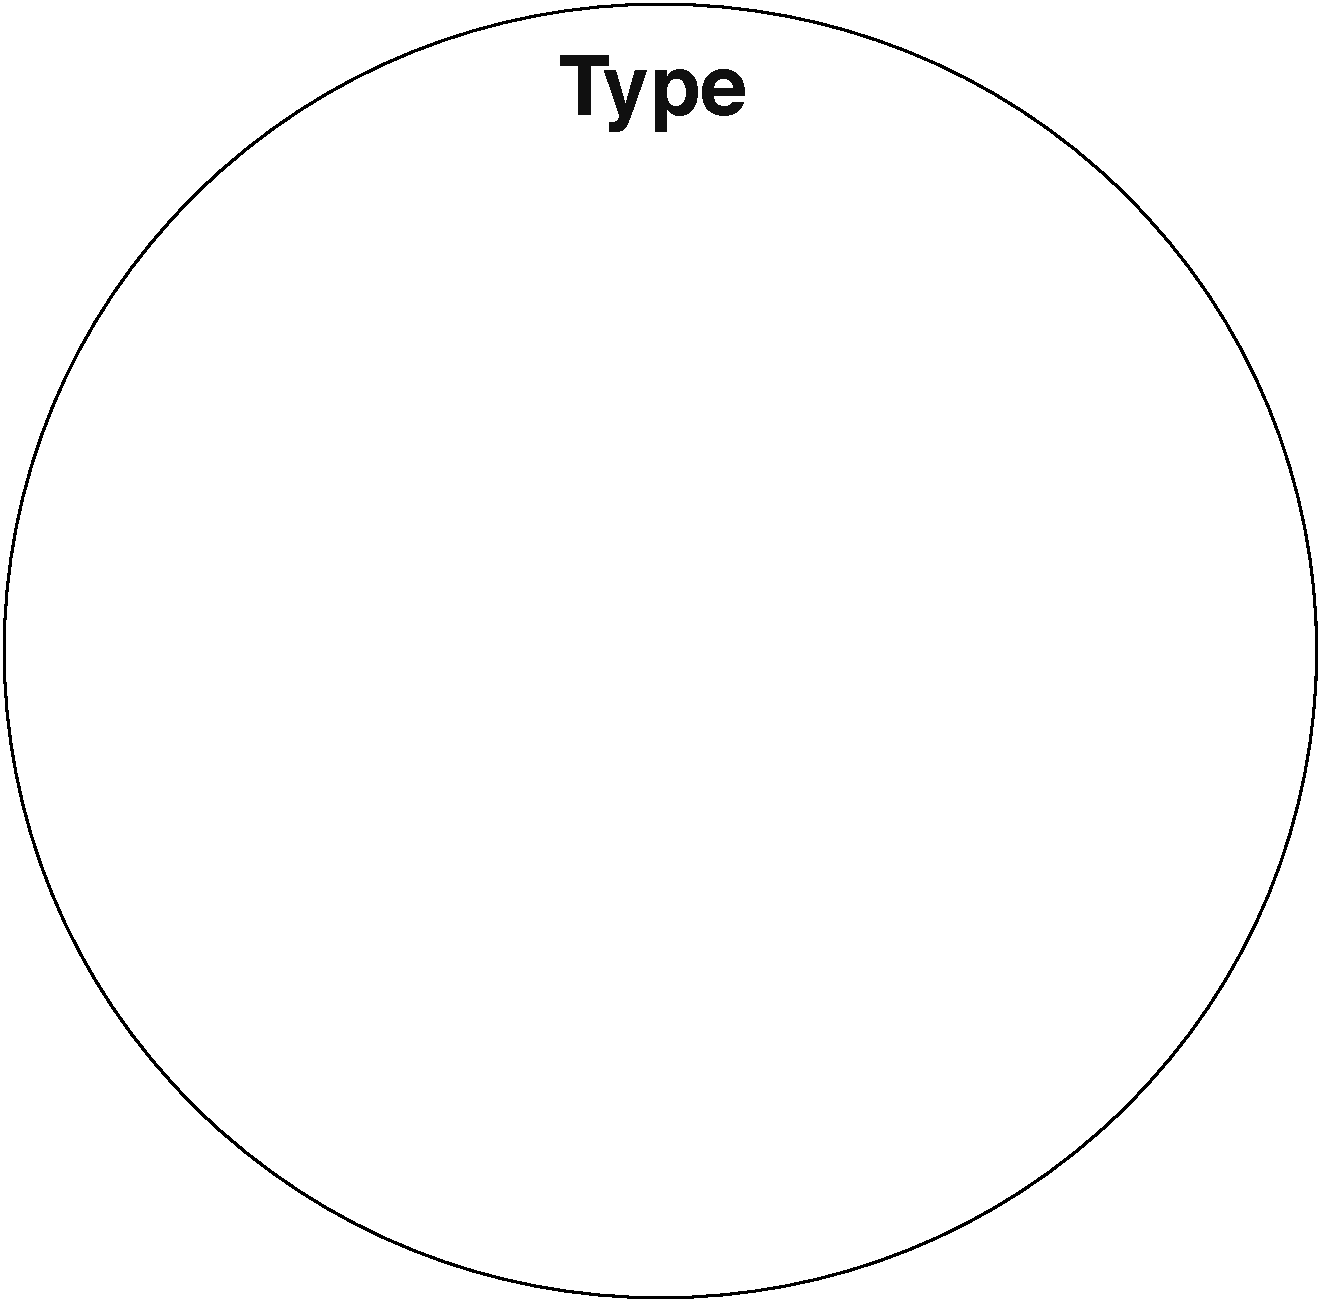
\includegraphics[width=2.8in]{universe-empty.pdf}
  \end{center}
\end{frame}

\begin{frame}
  \frametitle{Universes \`a la Tarski}
  \begin{center}
    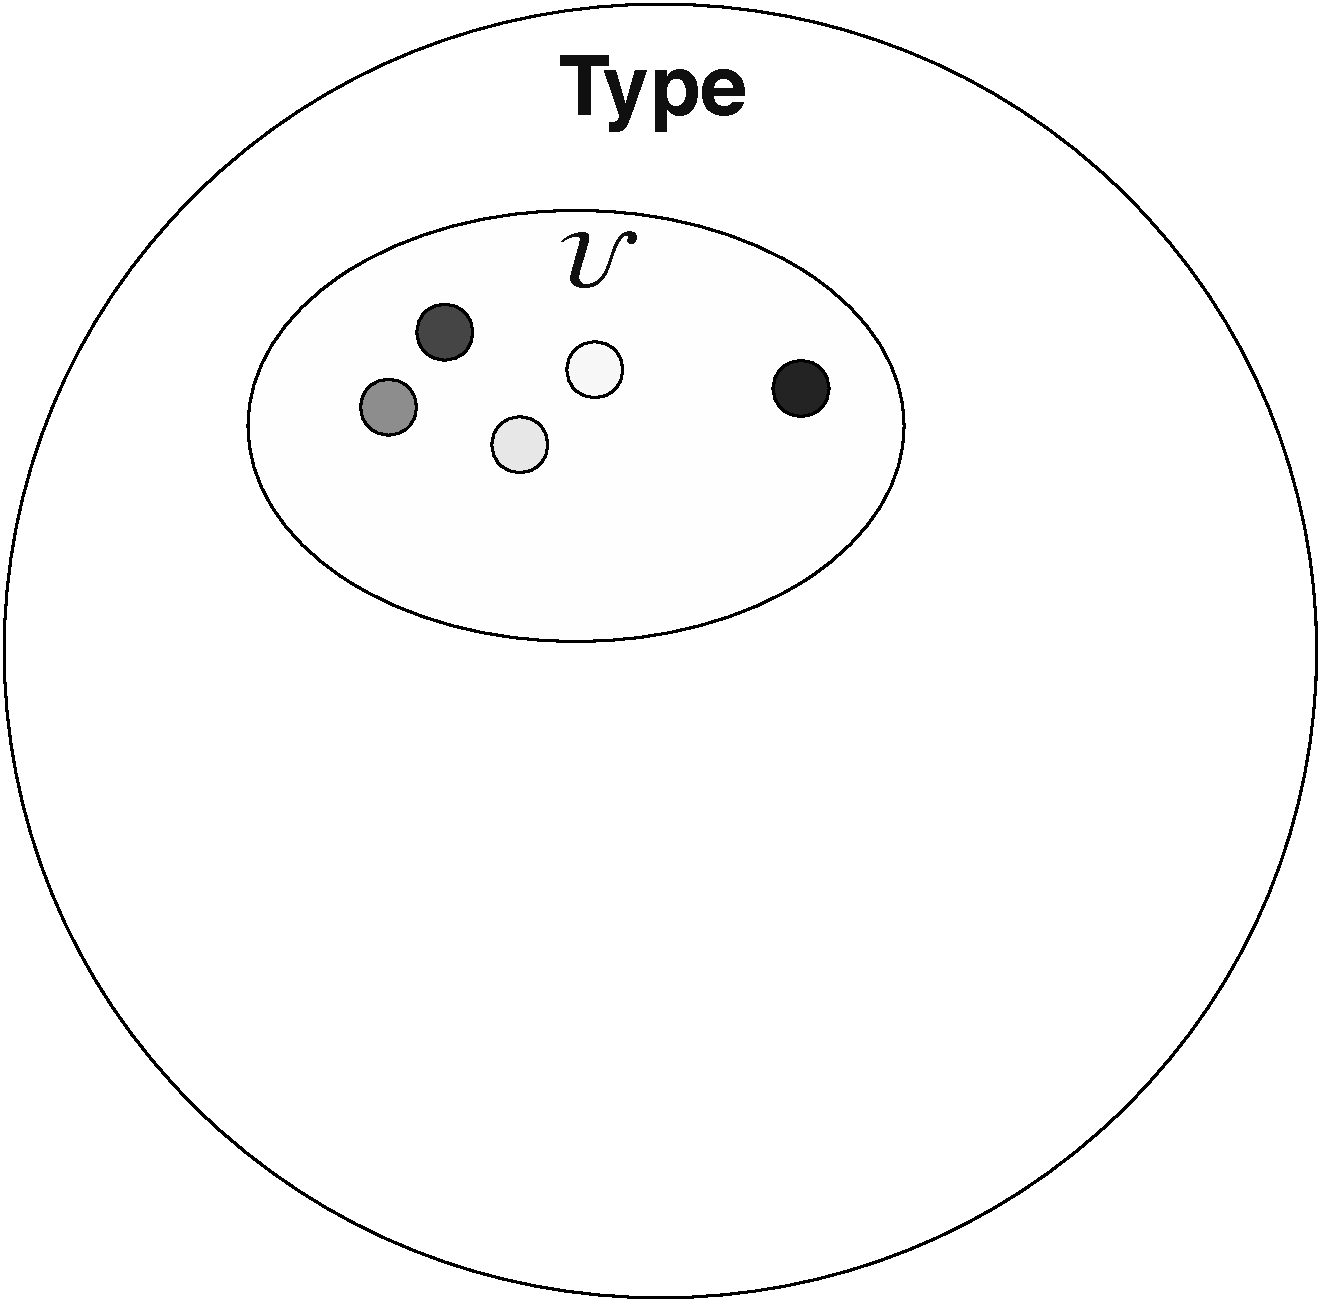
\includegraphics[width=2.8in]{universe-embedded.pdf}
  \end{center}
\end{frame}

\begin{frame}
  \frametitle{Universes \`a la Tarski}
  \begin{center}
    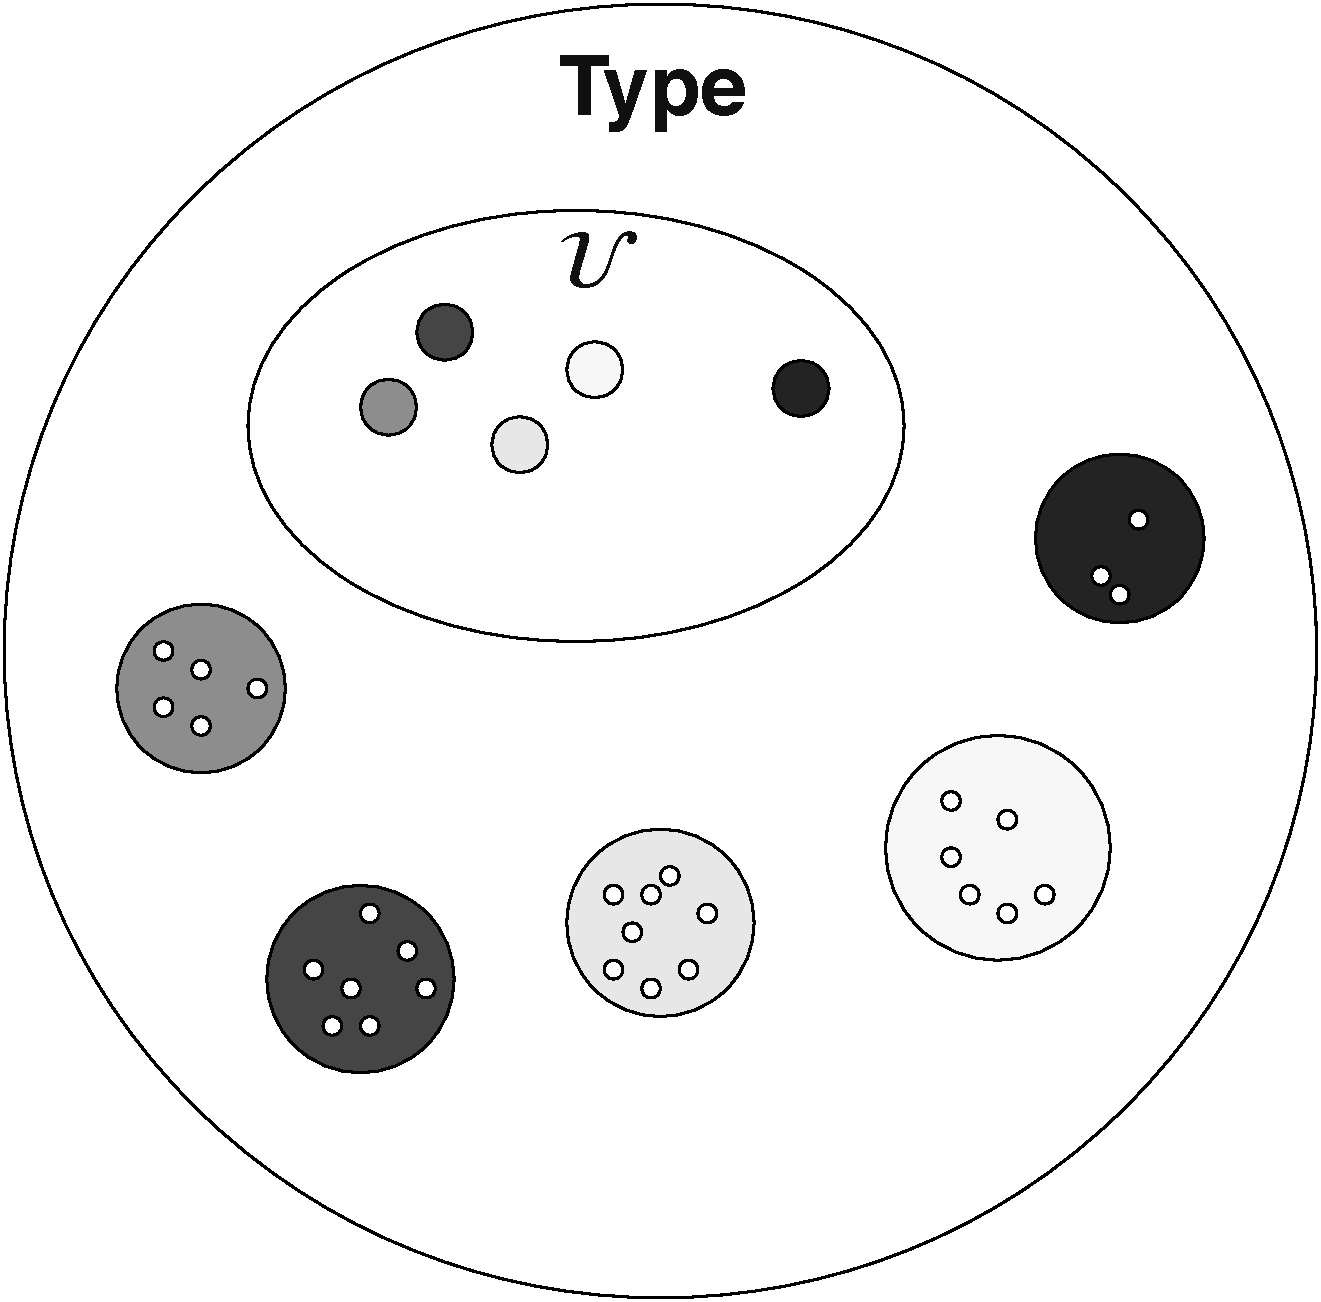
\includegraphics[width=2.8in]{universe-populated.pdf}
  \end{center}
\end{frame}

\begin{frame}
  \frametitle{Universes \`a la Tarski}
  \begin{center}
    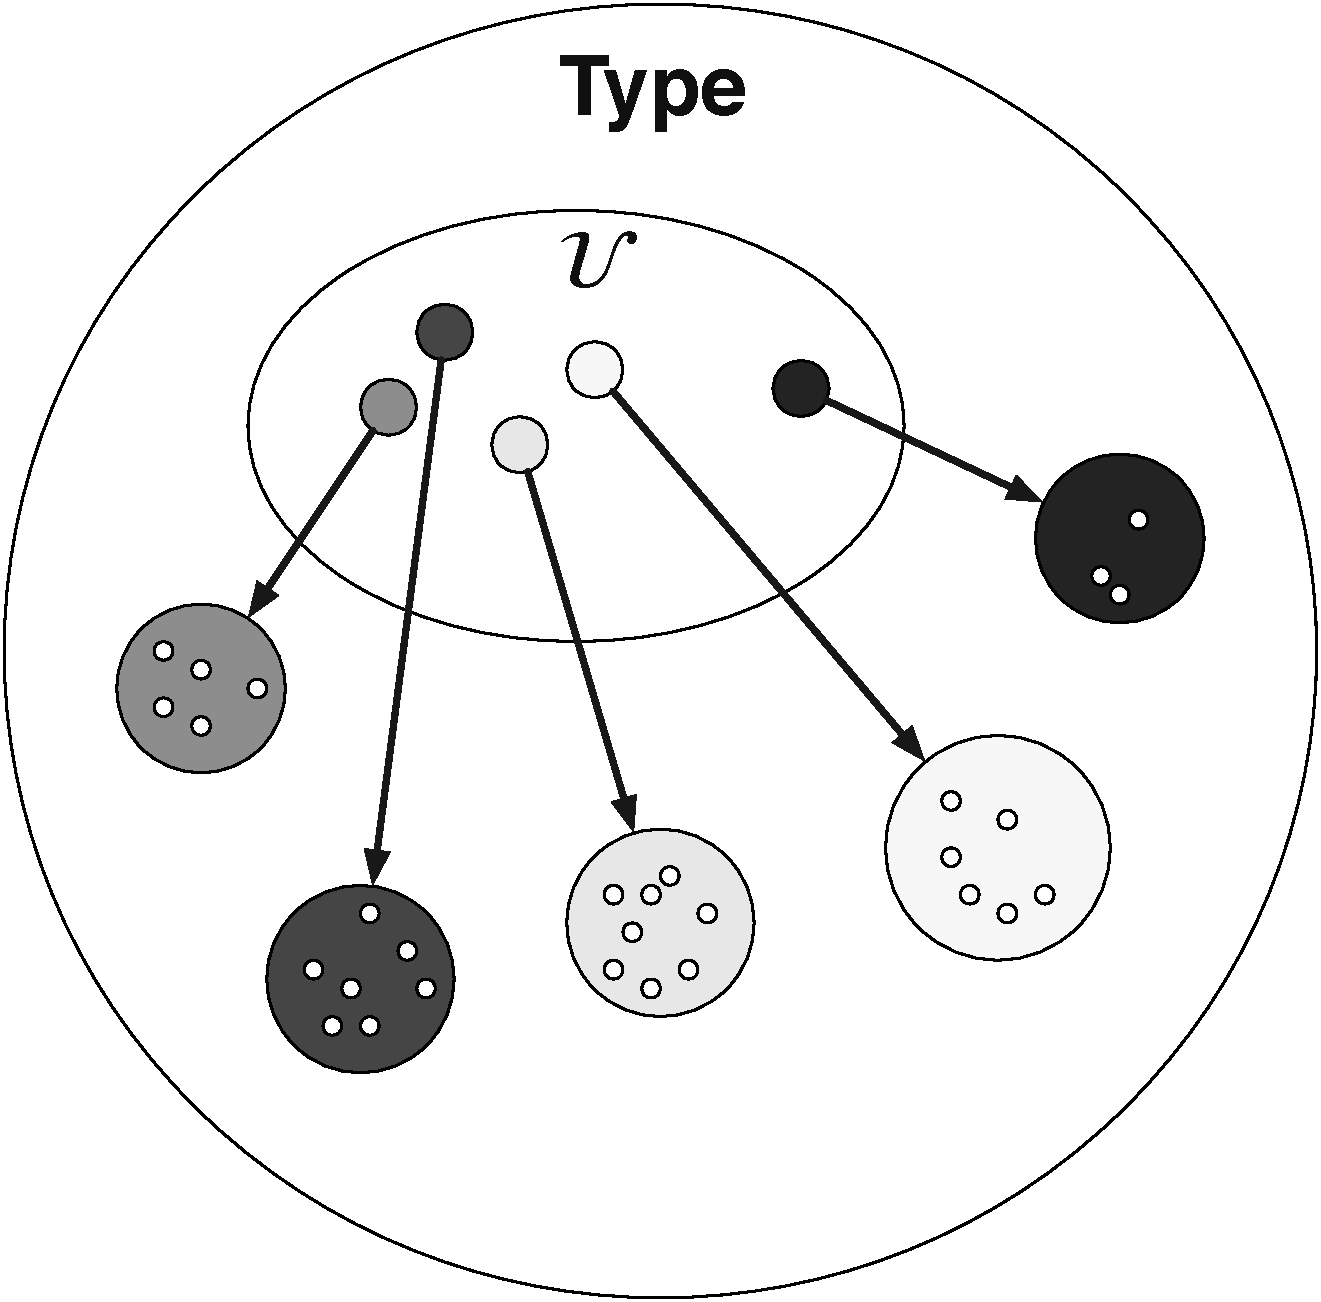
\includegraphics[width=2.8in]{universe-interpretation.pdf}
  \end{center}
\end{frame}

\begin{frame}[fragile]
  \frametitle{Records in Haskell}\pause
  \begin{lstlisting}
data Rec :: (|$\mathcal{U}$| -> *) -> [ |$\mathcal{U}$| ] -> * where |\pause|
  RNil :: Rec el|$_\mathcal{U}$| '[] |\pause|
  (:&) :: !(el|$_\mathcal{U}$| r) -> !(Rec el|$_\mathcal{U}$| rs) -> Rec el|$_\mathcal{U}$| (r ': rs)
  \end{lstlisting}
\end{frame}
\begin{frame}[fragile]
  \frametitle{Records in Haskell (Actually)}\pause

  \begin{lstlisting}
data TyFun :: * -> * -> *|\pause|
type family (f :: TyFun k l -> *) $ (x :: k) :: l|\pause|

data Rec :: (TyFun |$\mathcal{U}$| * -> *) -> [ |$\mathcal{U}$| ] -> * where
  RNil :: Rec el|$_\mathcal{U}$| '[]
  (:&) :: !(el|$_\mathcal{U}$| $ r) -> !(Rec el|$_\mathcal{U}$| rs) -> Rec el|$_\mathcal{U}$| (r ': rs)
  \end{lstlisting}
\end{frame}

\begin{frame}[fragile]
  \frametitle{Recovering HList}\pause
  \begin{lstlisting}
data Id :: (TyFun k k) -> * where
type instance Id $ x = x|\pause|

type HList rs = Rec Id rs|\pause|

ex :: HList [Int, Bool, String] |\pause|
ex = 34 :& True :& "vinyl" :& RNil
  \end{lstlisting}
\end{frame}

\section{Effectful Records}

\begin{frame}[fragile]
  \frametitle{Effects inside records}
  \begin{lstlisting}
data Rec :: (TyFun |$\mathcal{U}$| * -> *) -> (* -> *) -> [ |$\mathcal{U}$| ] -> * where
  RNil :: Rec el|$_\mathcal{U}$| f '[]
  (:&) :: !(f (el|$_\mathcal{U}$| $ r)) -> !(Rec el|$_\mathcal{U}$| f rs) -> Rec el|$_\mathcal{U}$| f (r ': rs)|\pause|

(=:) : Applicative f => sing r -> el|$_\mathcal{U}$| $ r -> Rec el|$_\mathcal{U}$| f '[r]|\pause|
k =: x = pure x :& RNil|\pause|

(<-:) : sing r -> f (el|$_\mathcal{U}$| $ r) -> Rec el|$_\mathcal{U}$| f '[r]|\pause|
k <-: x = x :& RNil
  \end{lstlisting}
\end{frame}

\begin{frame}[fragile]
  \frametitle{Compositional Kit}\pause

  \begin{lstlisting}
newtype Lift o f g x = Lift { runLift :: f x `o` g x }|\pause|

type Validator = Lift (->) Identity (Either Error)|\pause|
type JSONRenderer = Lift (->) Identity (Const Aeson.Pair)|\pause|

(<<*>>) :: Rec|$_\mathcal{U}$| (Lift (->) f g) rs -> Rec|$_\mathcal{U}$| f rs -> Rec|$_\mathcal{U}$| g rs|\pause|

rdist :: Applicative f => Rec|$_\mathcal{U}$| f rs -> f (Rec|$_\mathcal{U}$| Identity rs)|\pause|

rtraverse ::
  Applicative h
    => (f |$\leadsto$| h |$\circ$| g)
    -> Rec|$_\mathcal{U}$| f rs
    -> h (Rec|$_\mathcal{U}$| g rs)
  \end{lstlisting}
\end{frame}

\begin{frame}
  \centerline{\emph{\textbf{Demonstration}}}
\end{frame}

\end{document}

